\subsection{Sprint Plan}
\label{sec:projplan}

The project is organized in 4 regular sprints with each two weeks length. 

\begin{itemize}
\item 1st Sprint: \formatdate{14}{09}{2015} - \formatdate{25}{09}{2015}
\subitem Refinement of thesis concept
\subitem Implementation of prototype
\item 2nd Sprint: \formatdate{12}{10}{2015} - \formatdate{23}{10}{2015}
\subitem Development of algorithm
\subitem Development of Coupling Criteria catalog
\item 3rd Sprint: \formatdate{09}{11}{2015} - \formatdate{20}{11}{2015}
\subitem Finish functional requirements
\subitem Test significantly large project
\item 4th Sprint: \formatdate{30}{11}{2015} - \formatdate{11}{12}{2015}
\subitem Refine scoring system, fine tune sample models
\item 5th Sprint: \formatdate{14}{12}{2015} - \formatdate{18}{12}{2015} (one week)
\end{itemize}

The 5th sprint will solely be used to finish the documentation.

We utilized JIRA\cite{jira} to plan and organize the project. For every sprint we defined a set of stories which were, depending on their size, split into subtasks. Figure \ref{fig:jira} shows the number of stories ans subtasks created (green line) and resolved (red line) throughout the project timespan.

\begin{figure}[H]
	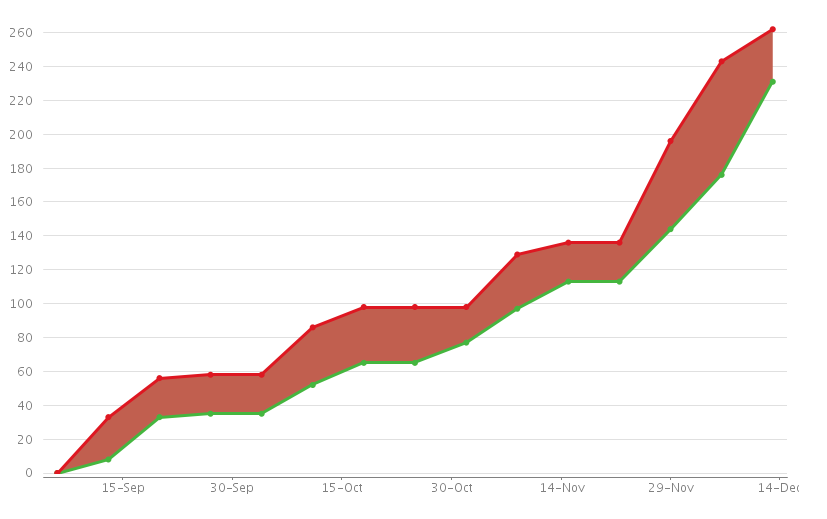
\includegraphics[scale=0.7]{images/jira.png}
	\caption{JIRA Stories and Substasks}
	\label{fig:jira}
\end{figure}

\subsection{Hours Worked}

We invested a total of 757 hours on this project. Michael Gysel worked 365 hours and Lukas Kölbener spent 392 hours on this thesis. Figure \ref{fig:hoursworked} breaks these numbers down into individual categories. We tracked them using epics in JIRA\cite{jira} which is a common technique in agile projects.

\begin{figure}[H]
	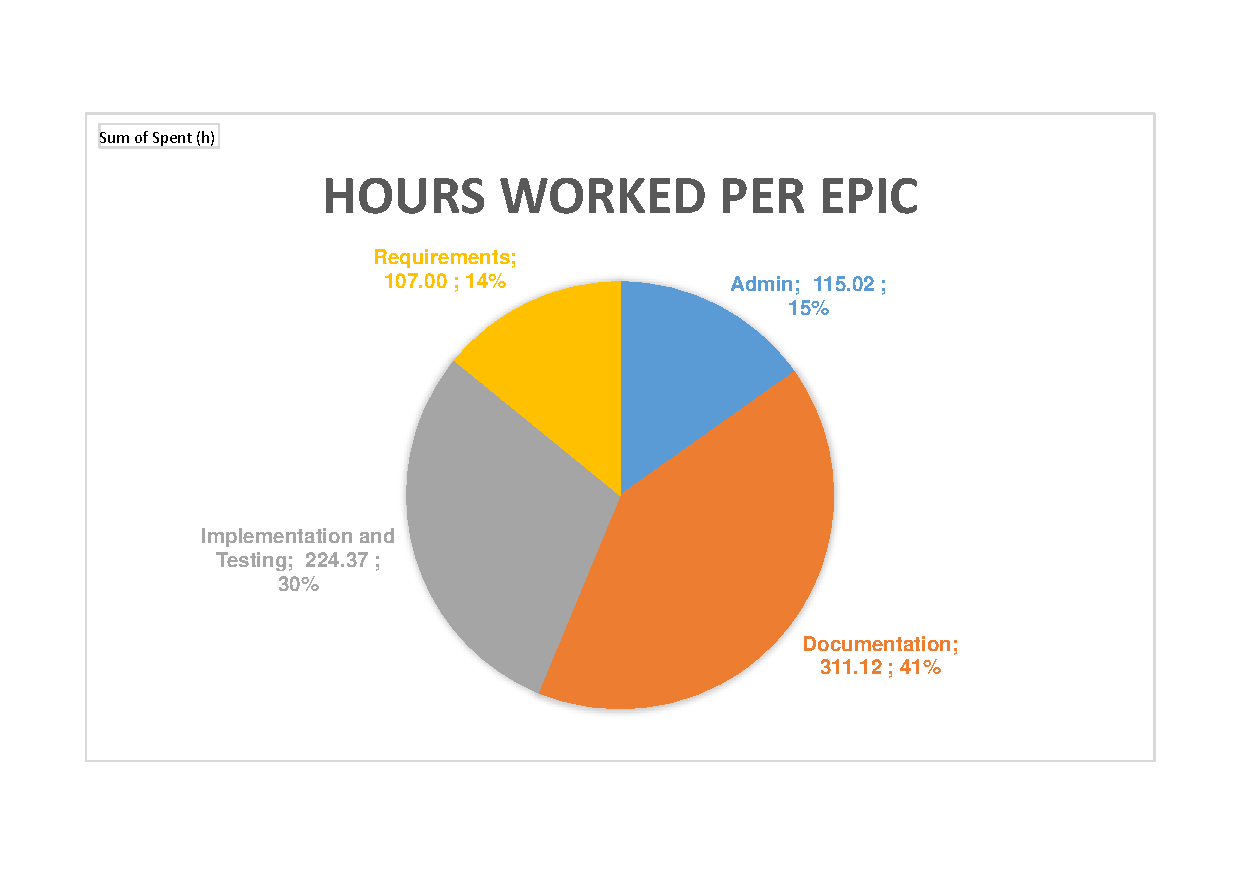
\includegraphics[scale=0.7]{diagrams/hoursperepic.pdf}
	\caption{Development Environment}
	\label{fig:hoursworked}
\end{figure}